
% !TEX encoding = UTF-8 Unicode 
% !TEX root = FieldGuide.tex


\Sec{Beta-Logistic Distribution}
\label{sec:BetaLogistic} 
\phantomsection
\addcontentsline{toc}{subsection}{~~~~~~~~~~~~Beta-Logistic} 
\phantomsection
\addcontentsline{toc}{subsection}{~~~~~~~~~~~~Standard Beta-Logistic}  



The {\bf beta-logistic } (Prentice, beta prime exponential, generalized logistic type IV, exponential generalized beta prime, exponential generalized beta type II, log-F, generalized F, Fisher-Z, generalized Gompertz-Verhulst type II) distribution~\cite{Prentice1976, McDonald1991, Johnson1995, Morton2000}
 is a four parameter, continuous, univariate, unimodal probability density, with infinite  support. The functional form in the most straightforward parameterization is
\begin{align}
\notag
\label{BetaLogistic}
\opr{BetaLogistic}(x\given  \pLoc, \pScale,\alpha,\gamma) 
& =
 \frac{1}{B(\alpha, \gamma) \Left| \pScale\Right|}
 \frac{e^{-\alpha \frac{x-\pLoc}{\pScale} }} { \Left(1 + e^{-\frac{x-\pLoc}{\pScale}  }\Right)^{\alpha+\gamma} } \checked
\\  &
\ x, \pLoc, \pScale,\alpha,\gamma \text{ in } {\mathbb R}
\\ \notag & \alpha,\gamma >0
\end{align}
The four real parameters consist of a location parameter $\pLoc$, a scale parameter $\pScale$, and two positive shape parameters $\alpha$ and $\gamma$.  The {\bf standard beta-logistic} distribution has zero location $\pLoc=0$ and unit scale $\pScale=1$.

The beta-logistic distribution is perhaps most commonly referred to as `generalized logistic', but this terminology is ambiguous, since many types of generalized logistic distribution have been investigated, and this distribution is not `generalized' in the same sense used elsewhere in this survey (See `generalized' \S \ref{sec:notation}). Therefore, we select the name `beta-logistic' as a less ambiguous terminology that mirrors the names beta, beta-prime, and beta-exponential.




\SSec{Special cases}

\dist{Burr type II} (generalized logistic type I, exponential-Burr, skew-logistic) distribution~\cite{Burr1942,Johnson1994}:
\begin{align}
\label{BurrII}
\opr{BurrII}(x\given \pLoc, \pScale,  \gamma) 
& = \frac{\gamma}{|\pScale|} \frac{e^{- \frac{x-\pLoc}{\pScale} } } { \Left(1 + e^{-\frac{x-\pLoc}{\pScale}  }\Right)^{\gamma+1} }
\checked
\\
& = \opr{BetaLogistic}(x\given \pLoc, \pScale, 1, \gamma) \checked
\notag
\end{align}

\begin{figure}[t!]
\begin{center}
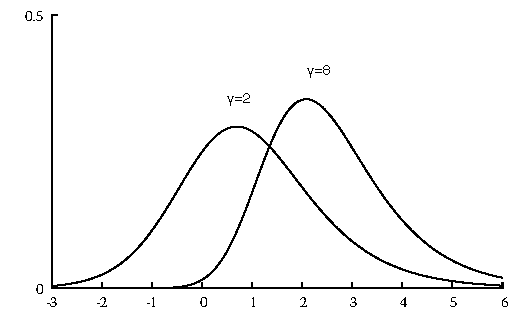
\includegraphics[width=\textwidth]{pdfBurrII}
\end{center}
\caption[Burr II distributions]{Burr type II distributions, $\opr{BurrII}(x\given0,1,\gamma)$}
\end{figure}


\dist{Reversed Burr type II} (generalized logistic type II) distribution~\cite{Johnson1994}:
\begin{align}
\label{RevBurrII}
\opr{RevBurrII}(x\given \alpha) 
& = \frac{\gamma}{|\pScale|}   \frac{e^{+ \frac{x-\pLoc}{\pScale} } } { \Left(1 + e^{+\frac{x-\pLoc}{\pScale}  }\Right)^{\gamma+1} }
\checked
\\
& = \opr{BurrII}(x\given \pLoc, -\pScale,  \gamma) \notag \checked \\
& = \opr{BetaLogistic}(x\given \pLoc, -\pScale, 1, \gamma) \notag \checked \\
& = \opr{BetaLogistic}(x\given \pLoc, +\pScale, \gamma, 1)  \notag \checked
\notag
\end{align}
By setting the $\lambda$ parameter to $1$ (instead of $\alpha$) we get a reversed Burr type II.


\begin{table*}[ptb] 
\begin{center}
\caption[Beta-logistic distribution -- Special cases]{Special cases of the beta-logistic distribution}
~\\
{\renewcommand{\arraystretch}{1.25} 
\begin{tabular}{llccccl}
\eqref{BetaLogistic} & Beta-Logistic & $\pLoc$ & $\pScale$ & $\alpha$ &  $\gamma$ \\
\hline  
\eqref{BurrII} & Burr type II					&. & . & 1 & . & \\
\eqref{RevBurrII}& Reversed Burr type II		&	. & . & . & 1 &\\
\eqref{CentralLogistic}& Central Logistic		&	. &   . & $\alpha$ & $\alpha$ & \\
\eqref{Logistic}& Logistic					& 	. & . & 1 & 1 & \\
\eqref{HyperbolicSecant}& Hyperbolic secant	&	. & . & $\tfrac{1}{2}$ & $\tfrac{1}{2}$ & \\
\end{tabular}
}
\end{center}
\end{table*}



% !TEX encoding = UTF-8 Unicode 
% !TEX root = FieldGuide.tex

\begin{table*}[p]
\caption[Beta-logistic distribution -- Properties]{Properties of the beta-logistic distribution}
\begin{align*}
\text{\hyperref[PropertiesSec]{Properties}}  \quad& \\
\text{notation} \quad &  \op{BetaLogistic}(x\given \pLoc,\pScale,\alpha,\gamma)  
\checked
\\
\text{PDF}\quad &  
\frac{1}{B(\alpha, \gamma) \Left| \pScale\Right|}
 \frac{e^{-\alpha \frac{x-\pLoc}{\pScale} }} { \Left(1 + e^{-\frac{x-\pLoc}{\pScale}  }\Right)^{\alpha+\gamma} }
\checked 
\\
\text{CDF / CCDF} \quad  &  
 \frac{B\big(\gamma, \alpha ;  ( 1+e^{-\frac{x-\pLoc}{\pScale}} )^{-1}  \big) }{B(\alpha,\gamma)}
& \pScale>0 \, \big/ \, \pScale<0 \checked
 \text{ \cite{\self}} \\
& \qquad  = I\big(  \gamma, \alpha;  ( 1+e^{-\frac{x-\pLoc}{\pScale}} )^{-1}  \big) \checked
\\
\text{parameters}\quad &   \pLoc,\ \pScale,\ \alpha, \gamma  \text{ in } \mathbb{R} \checked \\
& \alpha,\ \gamma >0 \checked
\\
\text{support} \quad &   x \in [-\infty,+\infty] \checked
\\
%\text{median} \quad  &  \cdots
%\\
%\text{mode} \quad  & \cdots
%\\
\text{mean} \quad  &  \pLoc +\pScale [ \psi(\gamma)-\psi(\alpha) ]  \checked %\cite{McDonnald1991} Has difference in scale sign
\\
\text{variance} \quad  & \pScale^2 [\psi_1(\alpha) + \psi_1(\gamma) ] \checked %\cite{McDonnald1991}
\\
\text{skew} \quad  &  \frac{ \psi_2(\gamma) - \psi_2(\alpha)}{[\psi_1(\alpha) + \psi_1(\gamma)]^{3/2}} \checked
\\
\text{kurtosis} \quad  &   \frac{\psi_3(\alpha) + \psi_3(\gamma)}{[\psi_1(\alpha) + \psi_1(\gamma)]^{2}} \checked
\\
%\text{entropy} \quad  & \cdots
%\\
\text{MGF} \quad  &  e^{ \pLoc t}\frac{\Gamma(\alpha-\pScale  t) \Gamma(\gamma+\pScale t)}{\Gamma(\alpha)\Gamma(\gamma)}
& \text{\cite{Johnson1995}} \checked
\\
\text{CF} \quad  &    e^{i \pLoc t} \frac{\Gamma(\alpha+ i \pScale  t) \Gamma(\gamma-i \pScale t)}{\Gamma(\alpha)\Gamma(\gamma)} \checked
\end{align*}
\end{table*}




\dist{Central logistic} (generalized logistic type III, inverse cosh, symmetric beta-logistic) distribution~\cite{Johnson1995}:
\begin{align}
\label{CentralLogistic}
\opr{CentralLogistic}(x\given \pLoc,\pScale,\alpha) 
& =
\frac{1}{B(\alpha, \alpha) |\pScale|}
 \frac{e^{-\alpha \frac{x-\pLoc}{\pScale} }} { \Left(1 + e^{-\frac{x-\pLoc}{\pScale}  }\Right)^{2\alpha} } \checked
  \\ \notag & = \frac{1}{B(\alpha, \alpha) |\pScale|} \bigl[\tfrac{1}{2} \op{sech} \Left(\tfrac{x-\pLoc}{2\pScale}  \Right)\bigr]^{2\alpha} 
  \checked 
\\ \notag & = \opr{BetaLogistic}(x\given \pLoc,\pScale,\alpha,\alpha) \checked
\end{align}
With equal shape parameters the beta-logistic is symmetric. This distribution limits to the Laplace distribution~\eqref{Laplace}.


\dist{Logistic} (sech-square, hyperbolic secant square, logit) distribution~\cite{Verhulst1845, Balakrishnan1991, Johnson1995}:
\begin{align}
\label{Logistic}
\opr{Logistic}(x\given \pLoc,\pScale) 
& =
 \frac{1}{ \Left| \pScale\Right|}
 \frac{e^{-\frac{x-\pLoc}{\pScale} }} { \Left(1 + e^{-\frac{x-\pLoc}{\pScale}  }\Right)^{2} }	\checked
 \\ \notag & = \frac{1}{4 |\pScale|} \op{sech}^2 \Left(\frac{x-\pLoc}{\pScale}  \Right)  \checked
 \\ \notag & = \opr{BetaLogistic}(x\given \pLoc,\pScale,1,1)	\checked
\end{align}





\dist{Hyperbolic secant} (inverse hyperbolic cosine, inverse cosh) distribution~\cite{Johnson1995,Perks1932,Talacko1956}:
\begin{align}
\label{HyperbolicSecant}
\opr{HyperbolicSecant}(x\given \pLoc, \pScale) 
& =
\frac{1}{\pi |\pScale|}
 \frac{1}{e^{+\sfrac{x-\pLoc}{2\pScale}} + e^{- \sfrac{x-\pLoc}{2\pScale} }} \checked
 \\ & = \frac{1}{2 \pi  |\pScale|} \op{sech}(\sfrac{x-\pLoc}{2\lambda}) \notag \checked
 \\ \notag & = \opr{BetaLogistic}(x\given  \pLoc, \pScale,\tfrac{1}{2},\tfrac{1}{2}) \checked
\end{align}
The hyperbolic secant cumulative distribution function features the Gudermannian sigmoidal function, $\op{gd}(z)$ . \index{Gudermannian function}
\begin{align*}
\op{HyperbolicSecantCDF}(x\given \pLoc, \pScale)  & = \frac{1}{\pi}\op{gd}(\frac{x-\pLoc}{2 \pScale}) \checked \\
& =  \frac{2}{\pi} \arctan(e^\frac{x-\pLoc}{2\pScale}) - \frac{1}{2} \checked
\end{align*}
The standardized hyperbolic secant distribution (zero mean, unit variance) is $\opr{HyperbolicSecant}(x\given 0, 1/\pi)\checked$.

\newcommand{\oo}{\infty}
\begin{figure}[t!]
\begin{center}
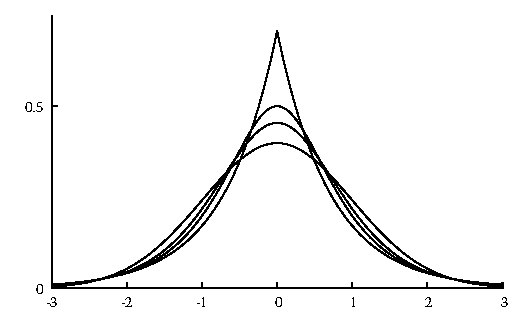
\includegraphics[width=\textwidth]{pdfSymBetaLogistic}
\end{center}
\caption[Central logistic distributions]{Special cases of the symmetric central logistic distribution~\eqref{CentralLogistic}: Standardized (zero mean, unit variance) normal~($\alpha\rightarrow\oo$), logistic~($\alpha=1$), hyperbolic secant~($\alpha=\tfrac{1}{2}$), and Laplace~($\alpha\rightarrow 0$)  (low to high peaks).}
\end{figure}




\SSec{Interrelations}
The beta-logistic distribution arises as a limit of the generalized beta prime distribution \secref{sec:BetaPrime}. The analogous limit of the generalized beta distribution leads to the beta-exponential family \secref{sec:BetaExp}. 


The beta-logistic distribution is the log transform of the beta prime distribution. 
\[
 \opr{BetaLogistic}(0,1,\alpha,\gamma)  \sim - \ln \opr{BetaPrime}(0,1,\alpha,\gamma)  \checked
 \notag
\] 
It follows that beta-logistic variates are related to ratios of gamma variates.
\[
\opr{BetaLogistic}(\pLoc,\pScale,\alpha,\gamma)  \sim \pLoc - \pScale \ln  \frac{\opr{StdGamma}_1(\gamma)}{\opr{StdGamma}_2(\alpha) }
\notag
\checked
\]


Negating the scale parameter is equivalent to interchanging the two shape parameters.
\[
\opr{BetaLogistic}(x\given \pLoc,+\pScale,\alpha,\gamma)  = \opr{BetaLogistic}(x\given \pLoc, - \pScale,\gamma,\alpha) \checked
\notag
\]



The beta-logistic distribution, with integer $\alpha$ and $\gamma$ is the logistic order statistics distribution~\cite{Birnbaum1963,Jones2004}~\secref{OrderStatistic}.  
\[
 \opr{OrderStatistic}_{\opr{Logistic}(\pLoc,\pScale)}  (x \given \gamma, \alpha ) =  \opr{BetaLogistic}(x\given \pLoc, \pScale, \alpha, \gamma) \checked
 \notag
\]


The beta-logistic limits to the gamma exponential~\eqref{GammaExp} and Laplace \eqref{Laplace} distributions.
\[
\opr{GammaExp}(x\given \nu, \lambda, \alpha)  & =
{\lim_{\gamma\rightarrow\infty} \opr{BetaLogistic}(x \given \nu+\lambda/\ln\gamma,\lambda, \alpha, \gamma)  }
\checked
\notag
\\
\opr{Laplace}(x\given \eta,\theta)   & = 
\lim_{\alpha\rightarrow 0} \opr{BetaLogistic}( x\given \eta, \theta\alpha\,\alpha,\alpha) \checked
\notag
\]



